\chapter{Tableur 1}\label{ficheTableur1}  

\begin{itemize}
\item Logiciel\footnote{Le logiciel LibreOffice est librement téléchargeable : \url{http://www.libreoffice.org/}} : \emph{LibreOffice Calc}
\item Prérequis : aucun
\item Matières concernées : mathématiques, physique-chimie, histoire-géographie
\item Objectifs : utiliser un tableur pour traiter des données, les visualiser sous forme de graphique et préparer un compte rendu au format PDF remis sur la plateforme \emph{Moodle}.
\item Compétences : 
        \begin{itemize}
        \item insérer une formule ;
        \item utiliser la recopie incrémentale ;
        \item tracer un graphique ;
        \item exporter au format PDF.
        \end{itemize}
\item Cette fiche est à réaliser :
        \begin{itemize}
        \item avant les vacances d'octobre en mathématiques ;
        \item avant les vacances de Noël en physique-chimie ;
        \item avant la fin du semestre de cours en histoire-géographie. 
        \end{itemize}
\prof{\item vous devez préparer un élément \underline{avant} la séance : un dossier de remise de devoir sur la page Moodle de votre classe car les élèves rendent cette activité sous la forme d'un fichier PDF déposé sur Moodle.}
\end{itemize}


\section{Introduction} 

Un tableur est un logiciel qui permet de faire des calculs à partir de tableaux contenant des nombres (les \emph{données}). Un tableur permet également de représenter ces données sous forme de graphiques qui en facilitent généralement la lecture.

\prof{on pourra ici indiquer qu'il existe plusieurs logiciels de tableur, le plus connu étant Excel contenu dans le pack Office de Microsoft. Le tableur utilisé ici est Calc, de la suite LibreOffice. Il présente l'avantage d'être libre et gratuit. L'utilisation de nombreuses fonctions est la même pour ces deux logiciels.}

\section{Ouvrir LibreOffice Calc}\index{Ouvrir!Calc}

Lancer le logiciel en utilisant la <<\,loupe\,>> :

\uneimageici{./images/generales/loupe}{.7\textwidth}

... puis en indiquant \emph{LibreOffice} :

\uneimageici{./images/generales/loupeRecherche}{.7\textwidth}

Choisir \emph{Classeur Calc} dans la liste proposée :

\uneimageici{./images/generales/fenetreOuverture}{.5\textwidth}

On arrive alors dans la fenêtre principale du tableur qui contient une \emph{feuille de calcul} vide :

\uneimageici{./images/tableur/CalcPresentation}{.9\textwidth}

\prof{Faites manipuler les cellules aux élèves, leur faire par exemple remplir la cellule \texttt{AA30} avec un nombre de leur choix, pour qu'ils doivent utiliser les ascenceurs. Montrez aux élèves comment redimensionner une colonne ou une ligne, plusieurs colonnes ou plusieurs lignes (en les sélectionnant auparavant), toutes les colonnes ou toutes les lignes (en les sélectionnant toutes).}


%
%
%  S  É  A  N  C  E     I
%
%





\section{Séance 1 : évolution des notes d'un élève}

\subsection{Énoncé}

\prof{assurez-vous que tous les élèves ont franchi les premières étapes ci-dessus. Lire ensuite l'énoncé avec les élèves et montrer le résultat attendu (affichage au TBI du résultat). À partir de ce point, les élèves travaillent chacun à leur rythme.}

\boiteEnonce{Au cours d'une année scolaire, un élève a obtenu les notes suivantes sur 20 points : \[11\quad 15\quad 12\quad 18\quad 16\quad 13\quad 10\quad 15\] On souhaite réaliser un graphique qui montre l'évolution de ses notes au cours de l'année et calculer ensuite sa moyenne annuelle.\newline Une fois votre travail terminé, vous devrez exporter votre fichier au format PDF (le fichier doit être nommé à partir de votre nom : \texttt{Nom-Prénom-date.pdf}) et le rendre sur la plateforme Moodle à l'endroit indiqué par votre enseignant.}

L'objectif est d'obtenir le résultat suivant :

\uneimageici{./images/tableur/CalcSituationFinaleMaths}{.75\textwidth}






\subsection{Entrer les données}

\begin{itemize}
\item Cliquer dans la cellule \texttt{A1}.
\item Taper au clavier le texte qui doit être contenu dans la cellule : \texttt{n\up{o} du test}.
\item Cliquer dans la cellule \texttt{B1} et écrire le premier numéro du test : 1.
\item Utiliser la \emph{recopie incrémentale}\index{Recopie incrémentale (Calc)}\index{Calc!Recopie incrémentale} pour remplir les cellules suivantes : pour cela, approcher le curseur de la souris du coin inférieur droit de la cellule \texttt{B1}. Lorsque le curseur se change en croix
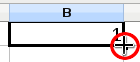
\includegraphics[scale=.4]{./images/tableur/recopieIncrementale}, cliquer et tirer (en maintenant cliqué) vers la droite pour remplir les cellules suivantes jusqu'à la valeur 8 (voir image ci-dessous).
\end{itemize}

\uneimageici{./images/tableur/recopieIncrementale2}{\textwidth}

\begin{itemize}
\item Cliquer dans la cellule \texttt{A2} et écrire \texttt{note sur 20}.
\item Remplir les cellules de la ligne 2 avec les notes correspondant aux différents tests.
\end{itemize}





\subsection{Sauvegarder le fichier}

Il est important de sauvegarder régulièrement le fichier sur lequel on travaille.


Pour enregistrer votre travail :
\begin{itemize}
\item Ouvrir le menu \texttt{Fichier}.
\item Choisir \texttt{Enregistrer sous...}
\item Choisir comme emplacement le \emph{Bureau} de l'ordinateur.
\item Entrer le nom du fichier sous la forme \texttt{Nom-Prénom-date.ods}
\end{itemize}

\uneimageici{./images/tableur/CalcEnregistrerFichier}{.8\textwidth}

Appuyer régulièrement sur la combinaison de touche \texttt{cmd} + \texttt{S} : c'est le \emph{raccourci clavier} permettant d'enregistrer votre travail.

\uneimageici{./images/generales/clavierCmdS}{.5\textwidth}



\cadre{\textbf{Différence entre \texttt{Enregistrer} et \texttt{Enregistrer sous...}}\newline Dans la plupart des logiciels, on peut : \begin{itemize}\item \textbf{enregistrer} le fichier sur lequel on travaille. Cette opération est possible si le fichier existe déjà et possède un nom. La version courante du fichier sera alors écrite en mémoire et remplacera l'ancienne version du fichier.\item \textbf{enregistrer sous...} le fichier sur lequel on travaille. Cette opération commence par demander un nouveau nom pour l'enregistrement du fichier. On peut donc ouvrir un fichier que l'on ne souhaite pas modifier, choisir \emph{enregistrer sous}, donner un nouveau nom et ainsi travailler sur une copie du fichier de départ.\item utiliser \texttt{cmd + S} (\emph{S} pour \emph{Save}) pour \textbf{enregistrer} le fichier courant. Bien que les documents soient enregistrés automatiquement par la majorité des logiciels, il faut régulièrement sauver son travail pour éviter les surprises.\end{itemize}}









\subsection{Créer un graphique}\index{Calc!Créer un graphique}\index{Créer un graphique (Calc)}

\begin{itemize}
\item Sélectionner les données à représenter : cliquer sur la cellule \texttt{B1} et tirer (en maintenant cliqué) jusqu'à la cellule \texttt{I2}. Les cellules sélectionnées apparaissent en bleu.
\uneimageici{./images/tableur/CalcCellulesSelectionnees}{.9\textwidth}

\item Cliquer alors sur l'icône diagramme\footnote{Pour créer un graphique, il est également possible de passer par le menu \texttt{Insertion} et choisir \texttt{Diagramme...} On retrouve alors la même boîte de dialogue.} 
\includegraphics[scale=.6]{./images/tableur/iconeDiagramme}.
\item Dans la boîte qui s'ouvre, choisir \texttt{XY (dispersion)}, puis le deuxième type proposé : \texttt{Points et lignes}.
\uneimageici{./images/tableur/CalcBoiteDiagramme1}{.6\textwidth}
\item Cliquer sur le bouton \texttt{Suivant} pour atteindre la partie de la boîte de dialogue qui concerne la \texttt{Plage de données}. Vérifier que le type \texttt{Séries de données en lignes} est bien coché (en effet, nos notes sont entrées en ligne).
\uneimageici{./images/tableur/CalcBoiteDiagramme2}{.6\textwidth}
\item Cliquer sur le bouton \texttt{Suivant} pour atteindre la partie de la boîte de dialogue qui concerne les \texttt{Séries de données}. Conserver les valeurs proposées par défaut.
\uneimageici{./images/tableur/CalcBoiteDiagramme3}{.6\textwidth}
\item Cliquer sur le bouton \texttt{Suivant} pour atteindre la partie de la boîte de dialogue qui concerne les \texttt{Éléments du diagramme}. Choisir un titre et les étiquettes (les <<\,noms\,>>) pour les axes $X$ et $Y$ avant de cliquer sur \texttt{Terminer}.
\uneimageici{./images/tableur/CalcBoiteDiagramme4}{.6\textwidth}
\end{itemize}

Vous avez maintenant un graphique qui s'est ajouté dans la feuille de calcul. Attention, la fenêtre du graphique est sélectionnée, ce qui est visible grâce aux huit poignées de sélection qui entourent la fenêtre :

\uneimageici{./images/tableur/CalcFenetreGraphiqueSelectionnee}{.6\textwidth}

Pour déplacer la fenêtre graphique, déplacer la souris sur le bord pour que le curseur prenne la forme d'une main (voir ci-dessus) : le déplacement s'effectue en maintenant cliqué et en déplaçant la souris. Pour revenir à la feuille de calcul, cliquer sur n'importe quelle cellule (les poignées de sélection disparaissent alors).









\subsection{Calculer la moyenne}\index{Moyenne (calcul de la)}\index{Calc!Moyenne (calcul de la)}

\begin{itemize}
\item Cliquer dans la cellule \texttt{A4} et entrer le texte : \texttt{Moyenne}.
\item Cliquer dans la cellule \texttt{B4} dans laquelle nous allons entrer une formule :
        \begin{itemize}
        \item taper un signe \texttt{=} qui signifie que la cellule va contenir une formule ;
        \item Taper le nom de la formule suivie d'une parenthèse ouvrante : \texttt{=MOYENNE(} ;
        \item à l'aide de la souris, sélectionner dans la feuille de calcul les cellules contenant les notes dont on veut calculer la moyenne (voir image ci-dessous) ;
        \uneimageici{./images/tableur/CalcCalculMoyenne}{.8\textwidth}
        \item appuyer sur la touche \texttt{Entrée} : la moyenne calculée apparaît.
        \end{itemize}
\end{itemize}




\subsection{Exporter au format PDF}\index{Calc!Exporter au format PDF}\index{PDF (exporter au format) (Calc)}

Une fois le travail achevé et sauvegardé, il faut exporter le fichier au format PDF. Pour cela, deux solutions :
\begin{itemize}\item passer par le menu \texttt{Fichier} et choisir \texttt{Exporter au format PDF...} Les réglages proposés par défaut dans la boîte de dialogue conviennent. Appuyer sur \texttt{Exporter} puis terminer en cliquant sur \texttt{Enregister}.\end{itemize} 

\deuximagesPGici{./images/texte/WriterMenuFichier}{.7\textwidth}%
                {./images/texte/WriterBoiteExportPDF}{\textwidth}

\begin{itemize}\item utiliser le bouton \texttt{Export direct au format PDF} :\end{itemize} 
\uneimageici{./images/texte/WriterIconePDF}{.3\textwidth}

Dans les deux cas, le fichier PDF est enregistré au même endroit que le fichier sur lequel on travaille.

\cadre{Le \textbf{format PDF} est un format parfaitement adapté aux échanges de documents : il est non modifiable et lisible sur tous les périphériques (ordinateurs, tablettes, smartphones). Il peut contenir du texte, des images, des liens vers l'internet et même des vidéos ou du son. \newline À chaque fois qu'il faut rendre ou envoyer un document qui n'est pas destiné à être modifié, il faut privilégier le format de fichier PDF.}  





\subsection{Remettre le travail achevé sur Moodle}

Une fois le travail terminé et exporté au format PDF, il faut le remettre au professeur. Pour cela, se connecter à la page \emph{Moodle} du cours. Chercher le dossier de remise de devoir (icône 
\includegraphics[width=.04\textwidth]{./images/methode/MoodleDevoirIcone1}), puis remettre le devoir. Si nécessaire, se reporter à la fiche méthode \emph{Remettre un devoir sur Moodle}, paragraphe \vref{MoodleRendreDevoir}.




\subsection{Pour aller plus loin...}

Après avoir terminé, faire des tests :

\begin{itemize}
\item modifier les notes et observer les modifications de la courbe ;
\item exporter le graphique en tant qu'image (sélectionner le graphique, maintenir la touche \texttt{cmd} enfoncée et cliquer sur le graphique, puis choisir \texttt{Exporter comme image...}) ;\index{Calc!Exporter un graphique comme image}\index{Exporter un graphique comme image (Calc)}
\item mettre en forme la feuille de calcul pour qu'elle ressemble à l'image présentée ci-dessous.
\end{itemize}


\uneimageici{./images/tableur/CalcPourAllerPlusLoin}{.7\textwidth}


%
%
%  S  É  A  N  C  E     II
%
%




\section{Séance 2 : Suivi en température d'une solidification}\label{ficheTableur2}

\prof{réalisez l'expérience avec vos élèves avant la séance, ou apportez le matériel correspondant à l'expérience pour donner du sens à la séance. De même, expliquez aux élèves les résultats obtenus. Il faut bien inciter les élèves à utiliser la recopie incrémentale pour générer les temps de 0 à 10 minutes.}

\uneimageici{./images/tableur/calcPhyChiSchema}{.4\textwidth}

\boiteEnonce{On place un tube à essai qui contient de l'eau distillée et un thermomètre dans un mélange réfrigérant. On relève alors la température de l'eau toutes les minutes. Les résultats obtenus sont reportés dans le tableau ci-dessous.
\begin{center}
\begin{tabular}{|c|c|c|c|c|c|c|c|c|c|c|c|}
\hline
temps $t$ (min) & 0 & 1 & 2 & 3 & 4 & 5 & 6 & 7 & 8 & 9 & 10 \\ \hline
température $T$ (\degre C) & 15 & 8 & 3 & 0 & 0 & 0 & 0 & 0 & $-1$ & $-3$ & $-5$ \\
\hline
\end{tabular}
\end{center}
On souhaite réaliser un graphique qui montre l'évolution de la température (en ordonnée) en fonction du temps (en abscisse).\newline Une fois votre travail terminé, vous devrez exporter votre fichier au format PDF (le fichier doit être nommé à partir de votre nom : \texttt{Nom-Prénom-date.pdf}) et le rendre sur la plateforme Moodle.
}

Le résultat à obtenir est présenté ci-dessous :

\uneimageici{./images/tableur/calcPhyChi}{.7\textwidth}




%
%
%  S  É  A  N  C  E     III
%
%




\section{Séance 3 : Évolution de la population mondiale}\label{ficheTableur3}

\boiteEnonce{La population mondiale au fil du temps est reportée dans le tableau ci-dessous.
\newline
\phantom{rien}
\newline
{\footnotesize
\begin{tabular}{|p{3.5cm}|c|c|c|c|c|c|c|c|c|c|}
\hline
Dates (années) & 0 & 400 & 1000 & 1500 & 1700 & 1800 & 1850 & 1900 & 1950 & 1980  \\ \hline
Population mondiale & \multirow{2}{*}{250} & \multirow{2}{*}{200} & \multirow{2}{*}{300} & \multirow{2}{*}{480} & \multirow{2}{*}{640} & \multirow{2}{*}{900} & \multirow{2}{*}{1300} & \multirow{2}{*}{1700} & \multirow{2}{*}{2700} & \multirow{2}{*}{4400} \\
 (en millions) & & & & & & & & & & \\   
\hline
\end{tabular}
%
\newline
\phantom{rien}
\newline
%
\begin{tabular}{|p{3.5cm}|c|c|c|c|c|c|}
\hline
Dates (années) & 1990 & 2000 & 2005 & 2010 & 2015 \\ \hline
Population mondiale & \multirow{2}{*}{5300} & \multirow{2}{*}{6100} & \multirow{2}{*}{6500} & \multirow{2}{*}{6900} & \multirow{2}{*}{7400} \\
(en millions) & & & & & \\  
\hline
\end{tabular}
} % fin du footnotesize tableau
%
\newline
{\tiny\emph{Source : Wikipédia (Population mondiale) et ONU (World Population Prospects http://esa.un.org/unpd/wpp/)}}
%
\newline
\phantom{rien}
\newline
On souhaite représenter l'évolution de la population mondiale depuis le début de notre ère. On veut afficher la population en millions d'individus (en ordonnée) en fonction de l'année (en abscisse).\newline Une fois votre travail terminé, vous devrez exporter votre fichier au format PDF (le fichier doit être nommé à partir de votre nom : \texttt{Nom-Prénom-date.pdf}) et le rendre sur la plateforme Moodle.
}

\prof{cette fois-ci les élèves ne voient pas le graphique à obtenir. Rappelez bien qu'il faut donner des noms aux axes (définir des étiquettes pour les axes), donner un titre au graphique. Interprétez avec les élèves le résultat obtenu. Le graphique que l'on doit obtenir est le suivant :\uneimageici{./images/tableur/calcHistoireGeoGraphique}{.7\textwidth}}
% il faut mettre un calcul de moyenne

% Pour aller plus loin : Europe vs Monde
